\documentclass[12pt,a4paper]{article}

\usepackage[margin=2.2cm]{geometry}
\usepackage{fontspec}
\IfFontExistsTF{Times New Roman}{\setmainfont{Times New Roman}}{\setmainfont{TeX Gyre Termes}}
\usepackage{amsmath,amssymb,bm}
\usepackage{booktabs}
\usepackage{float}
\usepackage{graphicx}
\usepackage{caption}
\usepackage{setspace}
\captionsetup{font=small,labelfont=bf,skip=4pt}
\graphicspath{{figures/}}
\usepackage{hyperref}
\setstretch{1.08}
\raggedbottom

\hypersetup{colorlinks=true,linkcolor=black,urlcolor=blue,pdftitle={}}

\begin{document}

Problem~5.13 closes a unity-feedback loop around a flexible plant with the lead compensator
\(D(s)=K(s+1)/(s+13)\).
The plant is a rigid-body double integrator with one undamped resonance at \(10~\mathrm{rad/s}\) and one undamped antiresonance at \(9~\mathrm{rad/s}\).
Parts (a)--(d) ask for the locus, for the damping that the locus can reach, for the gain that gives the dominant poles \(\zeta=0.707\), and for the step response at that gain.
The extension keeps the compensator fixed and asks two further questions.
What happens to the resonant branch when the plant antiresonance drifts up toward, and then past, the resonance?
Can a reference pre-filter remove the \(10~\mathrm{rad/s}\) ripple in the step response, and what does it do to the control signal?
The script is \texttt{hw06\_prob5\_13\_extension.m}. Every number below is taken from \texttt{simulation\_results.txt} (MATLAB R2022b), except three quantities computed separately from the closed-form expressions given with them: the real-axis break points, the stability scan over \(K\), and the reduced-model overshoots in Table~\ref{tab:os}.

%==============================================================================
\section{Loop transfer function and root-locus construction (Part a)}

The loop transfer function is
\begin{equation}
  L(s)=D(s)G(s)=K\,\frac{(s+1)(s^2+81)}{s^2(s+13)(s^2+100)},
  \label{eq:L}
\end{equation}
with open-loop poles \(0,0,-13,\pm j10\) and zeros \(-1,\pm j9\).
The closed-loop characteristic polynomial is
\begin{equation}
  s^5+13s^4+(100+K)s^3+(1300+K)s^2+81Ks+81K=0 .
  \label{eq:char}
\end{equation}
With \(n=5\) poles and \(m=3\) zeros, two branches go to infinity.
Their asymptotes leave the real axis at
\begin{equation}
  \sigma_a=\frac{\sum p_i-\sum z_i}{n-m}=\frac{-13-(-1)}{2}=-6,
  \qquad
  \phi_\ell=\pm 90^\circ .
  \label{eq:asym}
\end{equation}
The only real-axis segment is \(-13\le\sigma\le-1\): to its right lie the double pole at the origin and the zero at \(-1\), three real singularities in all, while the complex pairs contribute nothing to the count.

The double pole at the origin leaves vertically. For small \(K\) and small \(|s|\), \eqref{eq:L} reduces to \(L\approx 81K/(1300\,s^2)\), so the two roots start at
\(s\approx\pm j\sqrt{81K/1300}\).
At the resonant pole \(+j10\) the angle condition gives
\begin{align}
  \phi_{\mathrm{dep}}
  &=180^\circ+\bigl[\angle(j10+1)+\angle(j10-j9)+\angle(j10+j9)\bigr]\nonumber\\
  &\quad-\bigl[2\angle(j10)+\angle(j10+13)+\angle(j10+j10)\bigr]\nonumber\\
  &=180^\circ+\bigl[84.2894^\circ+90^\circ+90^\circ\bigr]-\bigl[180^\circ+37.5686^\circ+90^\circ\bigr]\nonumber\\
  &=136.7208^\circ .
  \label{eq:dep}
\end{align}
The script prints the two bracketed sums as \(264.2894^\circ\) and \(307.5686^\circ\), and the direction of the root at \(K=10^{-7}\) is \(136.7209^\circ\).
The same construction at the zero \(+j9\) gives an arrival angle of \(-138.9647^\circ\).
The resonant branch therefore leaves \(+j10\) up and to the left, swings around in the left half-plane, and enters \(+j9\) from the lower left.

On the real axis, \(dK/ds=0\) has two roots inside \([-13,-1]\).
The dominant pair, which left the origin vertically, comes back to the axis at a break-in point \(s=-2.314\) when \(K=53.13\). This matches the gain at which the script first finds \(\zeta_{\mathrm{dom}}=1\), \(K=53.1305\).
One of the two real roots then moves right to the zero at \(-1\).
The other moves left, meets the root coming from \(-13\) at the break-away point \(s=-5.315\) (\(K=59.06\)), and the pair leaves along the \(\sigma_a=-6\) asymptotes.
A root scan of \eqref{eq:char} over \(10^{-3}\le K\le 10^5\) finds all five roots in the open left half-plane, so the loop is stable for every positive gain in that range.

\begin{figure}[H]
  \centering
  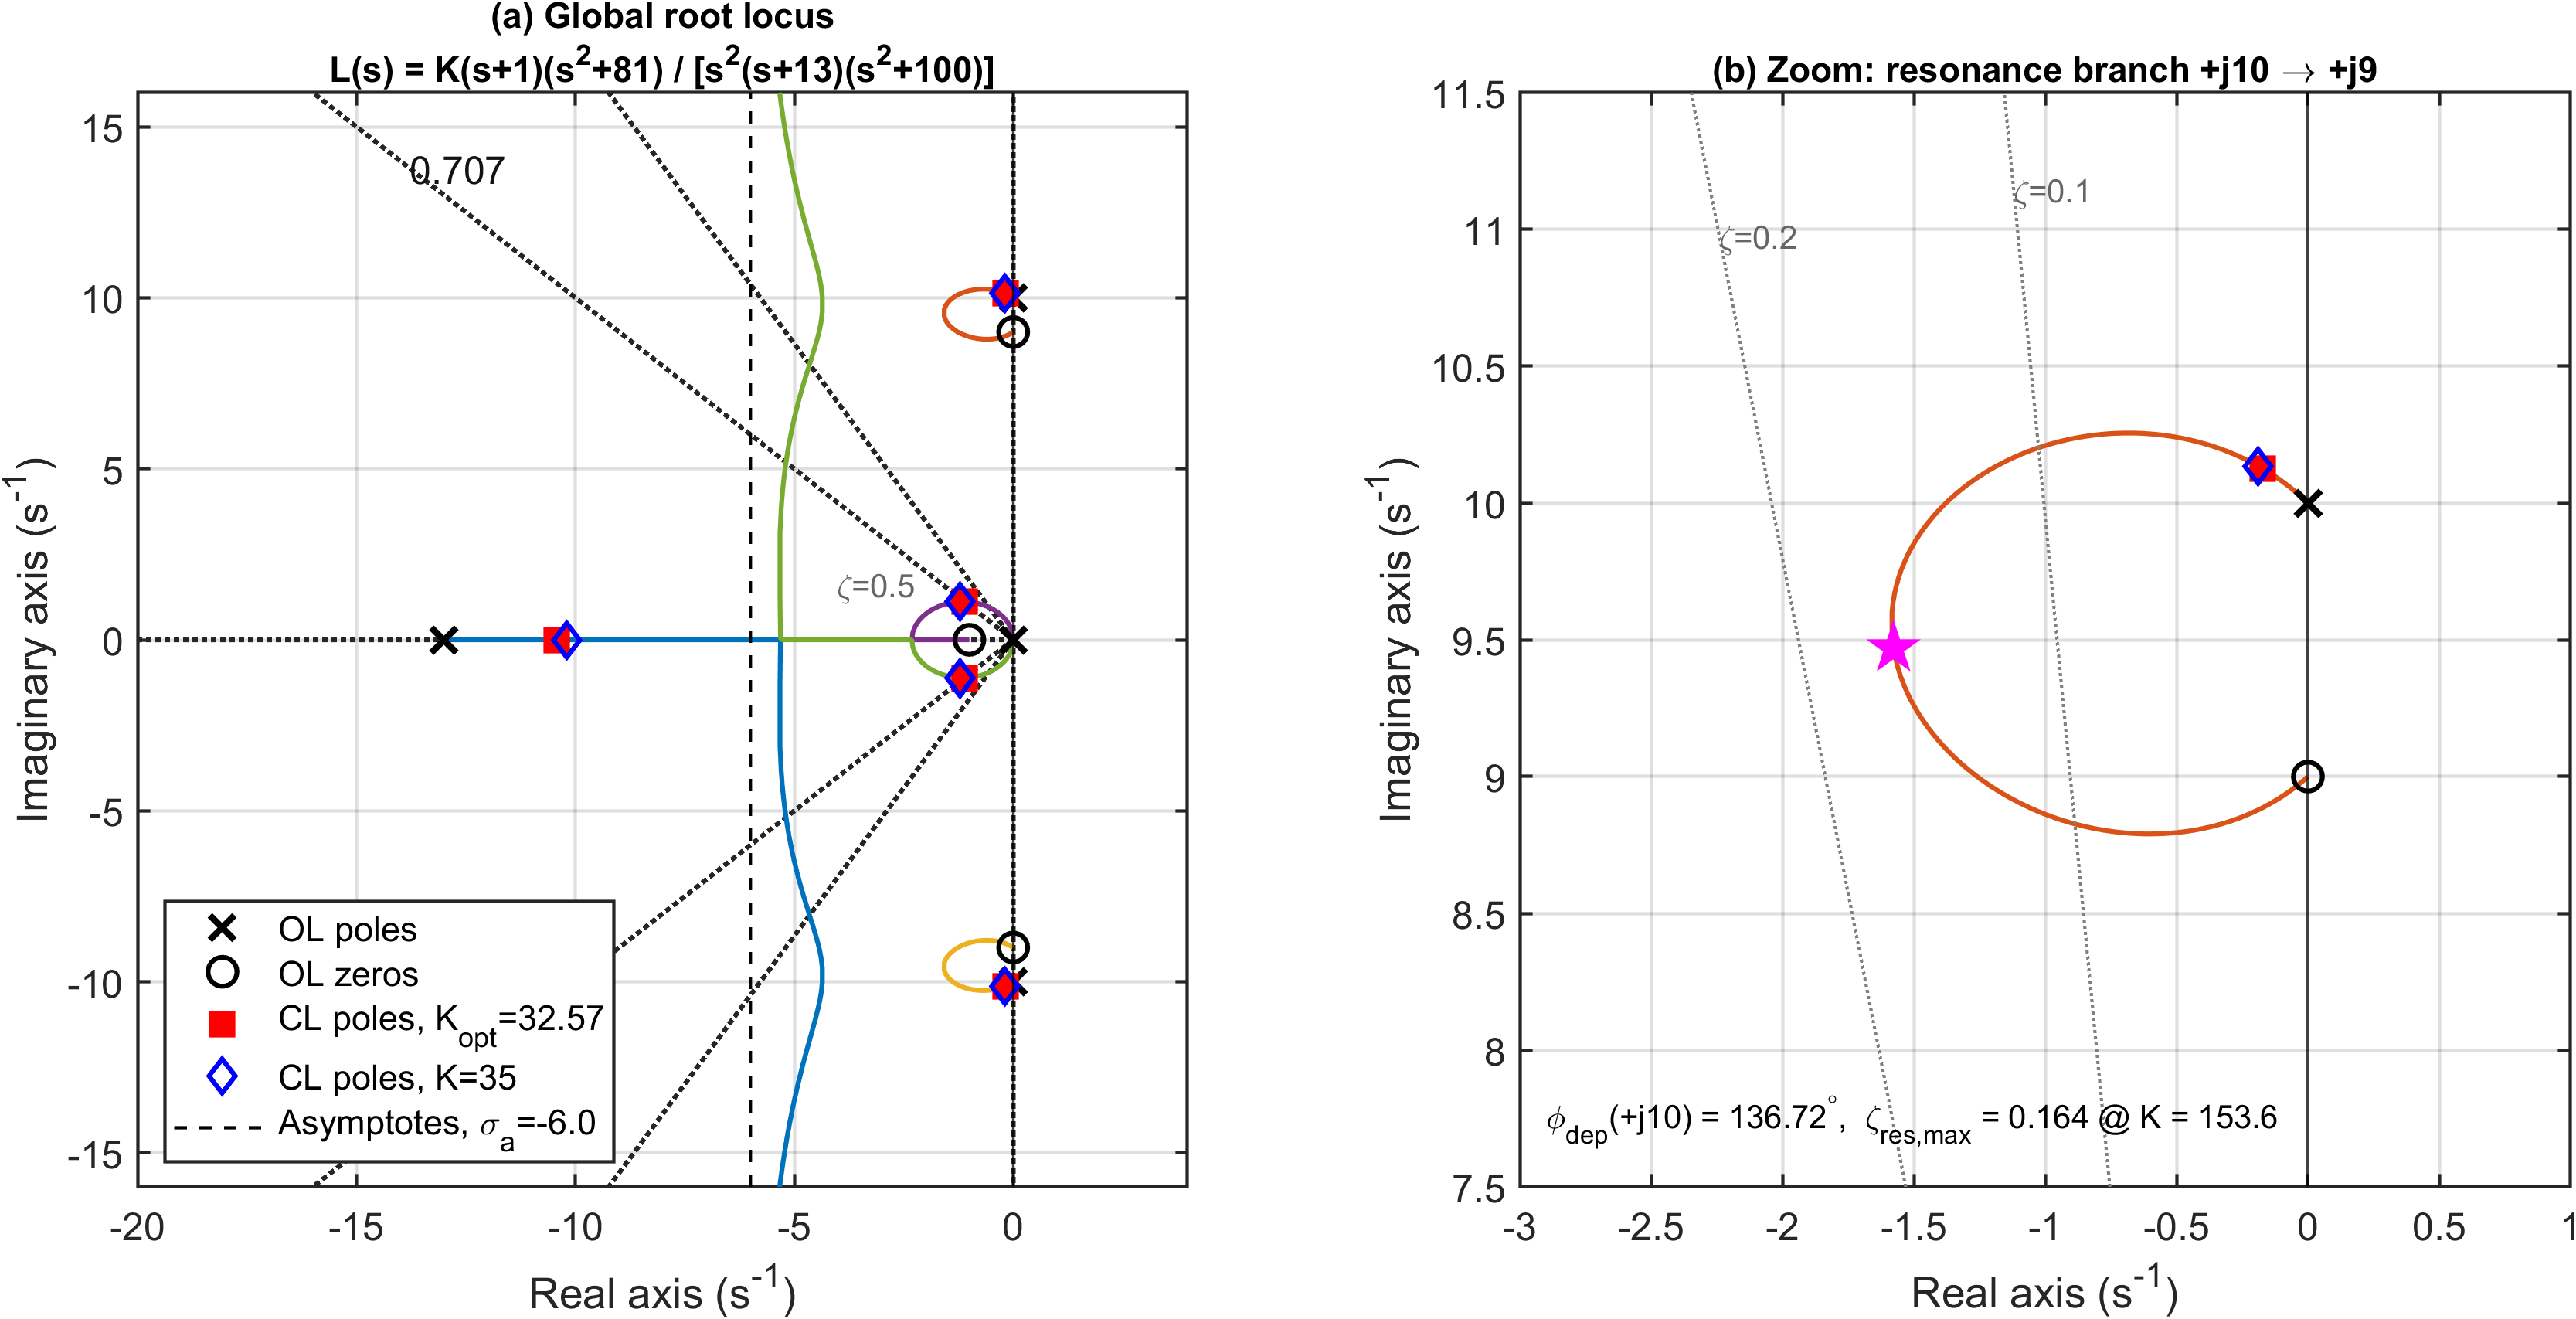
\includegraphics[width=\textwidth]{Fig1_RootLocus.png}
  \caption{(a) Root locus of \eqref{eq:L} with the \(\zeta=0.5\) and \(0.707\) rays.
  Red squares: closed-loop poles at \(K_{\mathrm{opt}}=32.57\). Blue diamonds: \(K=35\).
  (b) The resonant branch from \(+j10\) to \(+j9\). The star marks its most damped point, \(-1.5773+9.4694j\) at \(K=153.59\).}
  \label{fig:rl}
\end{figure}

%==============================================================================
\section{How much damping the locus allows (Part b)}

Table~\ref{tab:zeta} lists the damping ratios that each group of roots can reach.
The dominant pair has \(\zeta>0.5\) for \(17.62\le K\le 127.16\) and becomes real, \(\zeta=1\), at \(K=53.13\).
The resonant pair never gets past \(\zeta=0.1643\).
That maximum is reached at \(K=153.59\), and a second sweep over \(10^{-2}\le K\le 10^{5}\) finds the same value.
At \(K=10^5\) the resonant root is \(-0.0011+8.9990j\), already on top of the zero at \(+j9\).
The best value of the smallest damping ratio among all five roots is therefore also \(0.1643\), at the same gain.

\begin{table}[H]
  \centering
  \caption{Damping reachable on each branch group. The sweep is \(0.1\le K\le 200\) with \(50\,000\) points; the extended check runs to \(K=10^5\).}
  \label{tab:zeta}
  \begin{tabular}{lcc}
    \toprule
    Quantity & Value & Gain \\
    \midrule
    Dominant pair, \(\zeta>0.5\) & interval & \(17.62\le K\le 127.16\) \\
    Dominant pair, \(\zeta=1\) (break-in at \(-2.314\)) & \(1.0000\) & \(53.13\) \\
    Resonant pair, \(\zeta_{\max}\) & \(0.1643\) & \(153.59\) \\
    Resonant pair, \(\zeta_{\max}\) for \(10^{-2}\le K\le 10^{5}\) & \(0.1643\) & \(153.56\) \\
    \(\max_K\min(\zeta)\) over all five roots & \(0.1643\) & \(153.59\) \\
    \bottomrule
  \end{tabular}
\end{table}

The answer to Part~(b) is therefore no.
A gain exists that gives the dominant poles \(\zeta>0.5\), but no gain does that for the resonant pair, so no gain gives all roots \(\zeta>0.5\).
The reason is visible in Figure~\ref{fig:rl}(b).
The resonant branch begins at \(+j10\) and ends at \(+j9\), so it is a closed loop trapped between the pole and the zero.
In this run it never goes further left than \(\sigma=-1.58\) while staying above \(\omega\approx 8.8\), and \(1.58/9.6\approx 0.16\) is the most damping that region can hold.
The width of the loop is set by how far apart the pole and the zero are, not by \(K\): a larger gain only drives the root into the zero at \(+j9\), where the damping returns to zero.

%==============================================================================
\section{Gain for dominant damping 0.707 (Part c)}

Solving \(\zeta_{\mathrm{dom}}(K)=\sqrt2/2\) with \texttt{fzero} gives
\begin{equation}
  K_{\mathrm{opt}}=32.5673 .
  \label{eq:Kopt}
\end{equation}
The textbook value \(K\approx 35\) was read from \texttt{rlocfind}, a graphical pick, and gives \(\zeta_{\mathrm{dom}}=0.7389\) instead.
Table~\ref{tab:cl} lists both sets of closed-loop poles.
The difference between the two gains matters little: the dominant natural frequency changes from \(1.570\) to \(1.645~\mathrm{rad/s}\), and the resonant damping changes from \(0.0170\) to \(0.0186\).

\begin{table}[H]
  \centering
  \caption{Closed-loop poles and unit-step metrics. \(t_r\) is the \(10\)--\(90\%\) rise time, \(t_s\) uses the \(2\%\) band, and \(A_{\mathrm{res}}\) is the initial amplitude \(2|\mathrm{Res}|\) of the resonant mode in \(y(t)\).}
  \label{tab:cl}
  \small
  \begin{tabular}{lcc}
    \toprule
    Quantity & \(K_{\mathrm{opt}}=32.5673\) & \(K=35\) \\
    \midrule
    Dominant pair & \(-1.1101\pm1.1101j\) & \(-1.2158\pm1.1086j\) \\
    \(\zeta_{\mathrm{dom}}\), \(\omega_{n,\mathrm{dom}}\) & \(0.7071\), \(1.5699~\mathrm{rad/s}\) & \(0.7389\), \(1.6454~\mathrm{rad/s}\) \\
    Resonant pair & \(-0.1725\pm10.1262j\) & \(-0.1885\pm10.1349j\) \\
    \(\zeta_{\mathrm{res}}\), \(\omega_{n,\mathrm{res}}\) & \(0.0170\), \(10.1276~\mathrm{rad/s}\) & \(0.0186\), \(10.1367~\mathrm{rad/s}\) \\
    Real pole & \(-10.4347\) & \(-10.1914\) \\
    \midrule
    \%OS & \(28.83\%\) & \(28.17\%\) \\
    \(t_r\), \(t_p\) & \(0.548~\mathrm{s}\), \(1.448~\mathrm{s}\) & \(0.529~\mathrm{s}\), \(1.437~\mathrm{s}\) \\
    \(t_s\) (\(2\%\)) & \(5.522~\mathrm{s}\) & \(5.497~\mathrm{s}\) \\
    \(A_{\mathrm{res}}\) & \(0.0477\) & \(0.0522\) \\
    \bottomrule
  \end{tabular}
\end{table}

%==============================================================================
\section{Step response (Part d)}

The step response is shown as Design~A in Figure~\ref{fig:pf}. It consists of a well-damped rise with a \(10~\mathrm{rad/s}\) ripple on top, as in the textbook solution.
Two of its numbers would be misread if the dominant pair were treated as a standard second-order system.

The first is the overshoot.
A pair with \(\zeta=0.739\) alone overshoots by only \(e^{-\pi\zeta/\sqrt{1-\zeta^2}}=3.19\%\).
The measured value is \(28.17\%\).
The difference comes from the closed-loop zero at \(s=-1\), which the lead compensator puts into \(T(s)=K(s+1)(s^2+81)/\Delta(s)\).
That zero is closer to the origin than the dominant poles, \(|s|=1.645\), so it adds a derivative-like term to the step response.
Table~\ref{tab:os} adds the factors of \(T(s)\) one at a time, each time scaled to unit dc gain.

\begin{table}[H]
  \centering
  \caption{Overshoot decomposition at \(K=35\). The first three rows are reduced models built from the poles in Table~\ref{tab:cl}; the last row is the simulated full loop.}
  \label{tab:os}
  \begin{tabular}{lcc}
    \toprule
    Model & \%OS & \(t_p\) \\
    \midrule
    Dominant pair only & \(3.19\%\) & \(2.834~\mathrm{s}\) \\
    \(+\) zero at \(-1\) & \(24.90\%\) & \(1.244~\mathrm{s}\) \\
    \(+\) real pole at \(-10.19\) & \(24.53\%\) & \(1.354~\mathrm{s}\) \\
    Full \(T(s)\) (simulation) & \(28.17\%\) & \(1.437~\mathrm{s}\) \\
    \bottomrule
  \end{tabular}
\end{table}

The zero alone accounts for about \(22\) of the \(28\) percentage points, and it also halves the peak time.
The remaining \(3.6\) points come from the resonant mode adding to the peak.
Specifying \(\zeta=0.707\) for the dominant pair therefore does not give the \(4.3\%\) overshoot that the second-order formula promises for this loop.

The second is the settling time.
The resonant mode starts with amplitude \(A_{\mathrm{res}}=0.0522\) and decays as \(e^{-0.1885t}\).
That envelope stays above the \(2\%\) band until
\begin{equation}
  t=\frac{\ln(0.0522/0.02)}{0.1885}=5.09~\mathrm{s},
  \label{eq:tsenv}
\end{equation}
while the dominant envelope \(e^{-1.216t}\) has dropped below \(e^{-6}\) by then.
The simulated \(t_s=5.497~\mathrm{s}\) is therefore set by the vibration, not by the dominant pair. The envelope gives a lower bound because the other modes have not vanished completely near \(5~\mathrm{s}\).
In this loop, raising \(\zeta_{\mathrm{dom}}\) would not shorten \(t_s\) unless the residual \(10~\mathrm{rad/s}\) mode is also addressed.

%==============================================================================
\section{Extension 1: antiresonance drift and pole--zero flip}

The plant zero \(s^2+\omega_z^2\) is the antiresonance of a collocated sensor and actuator, and it moves when the structure is loaded.
Three values of \(\omega_z\) are tested with the compensator and \(K=35\) held fixed: the nominal \(\omega_z=9\), a near-cancellation value \(\omega_z=9.798\), and a flipped value \(\omega_z=10.247\) above the resonance \(\omega_p=10\).

Only one term of \eqref{eq:dep} depends on \(\omega_z\): the angle from the zero \(+j\omega_z\) to the pole \(+j10\).
It is \(+90^\circ\) while \(\omega_z<10\) and \(-90^\circ\) once \(\omega_z>10\); every other angle is unchanged.
Crossing \(\omega_z=\omega_p\) therefore subtracts exactly \(180^\circ\) from the departure angle,
\begin{equation}
  \phi_{\mathrm{dep}}\big|_{\omega_z>\omega_p}=136.7208^\circ-180^\circ=-43.2792^\circ ,
  \label{eq:flip}
\end{equation}
which is the value the script prints. The numerical check at \(K=10^{-7}\) gives \(-43.2778^\circ\).
The sign of \(\cos\phi_{\mathrm{dep}}\) decides which half-plane the resonant root moves into at small gain. It moves left for \(136.7^\circ\) and right for \(-43.3^\circ\).

\begin{table}[H]
  \centering
  \caption{Resonant root at \(K=35\) for three antiresonance frequencies.}
  \label{tab:flip}
  \small
  \begin{tabular}{lccccc}
    \toprule
    Case & \(\omega_z\) & \(\phi_{\mathrm{dep}}\) & Resonant root & \(A_{\mathrm{res}}\) & Stable \\
    \midrule
    1: nominal & \(9.0000\) & \(136.72^\circ\) & \(-0.18848\pm10.13493j\) & \(0.0522\) & yes \\
    2: near cancellation & \(9.7980\) & \(136.72^\circ\) & \(-0.04115\pm10.02722j\) & \(0.0113\) & yes \\
    3: flipped & \(10.2470\) & \(-43.28^\circ\) & \(+0.05248\pm9.96699j\) & \(0.0144\) & no \\
    \bottomrule
  \end{tabular}
\end{table}

\begin{figure}[H]
  \centering
  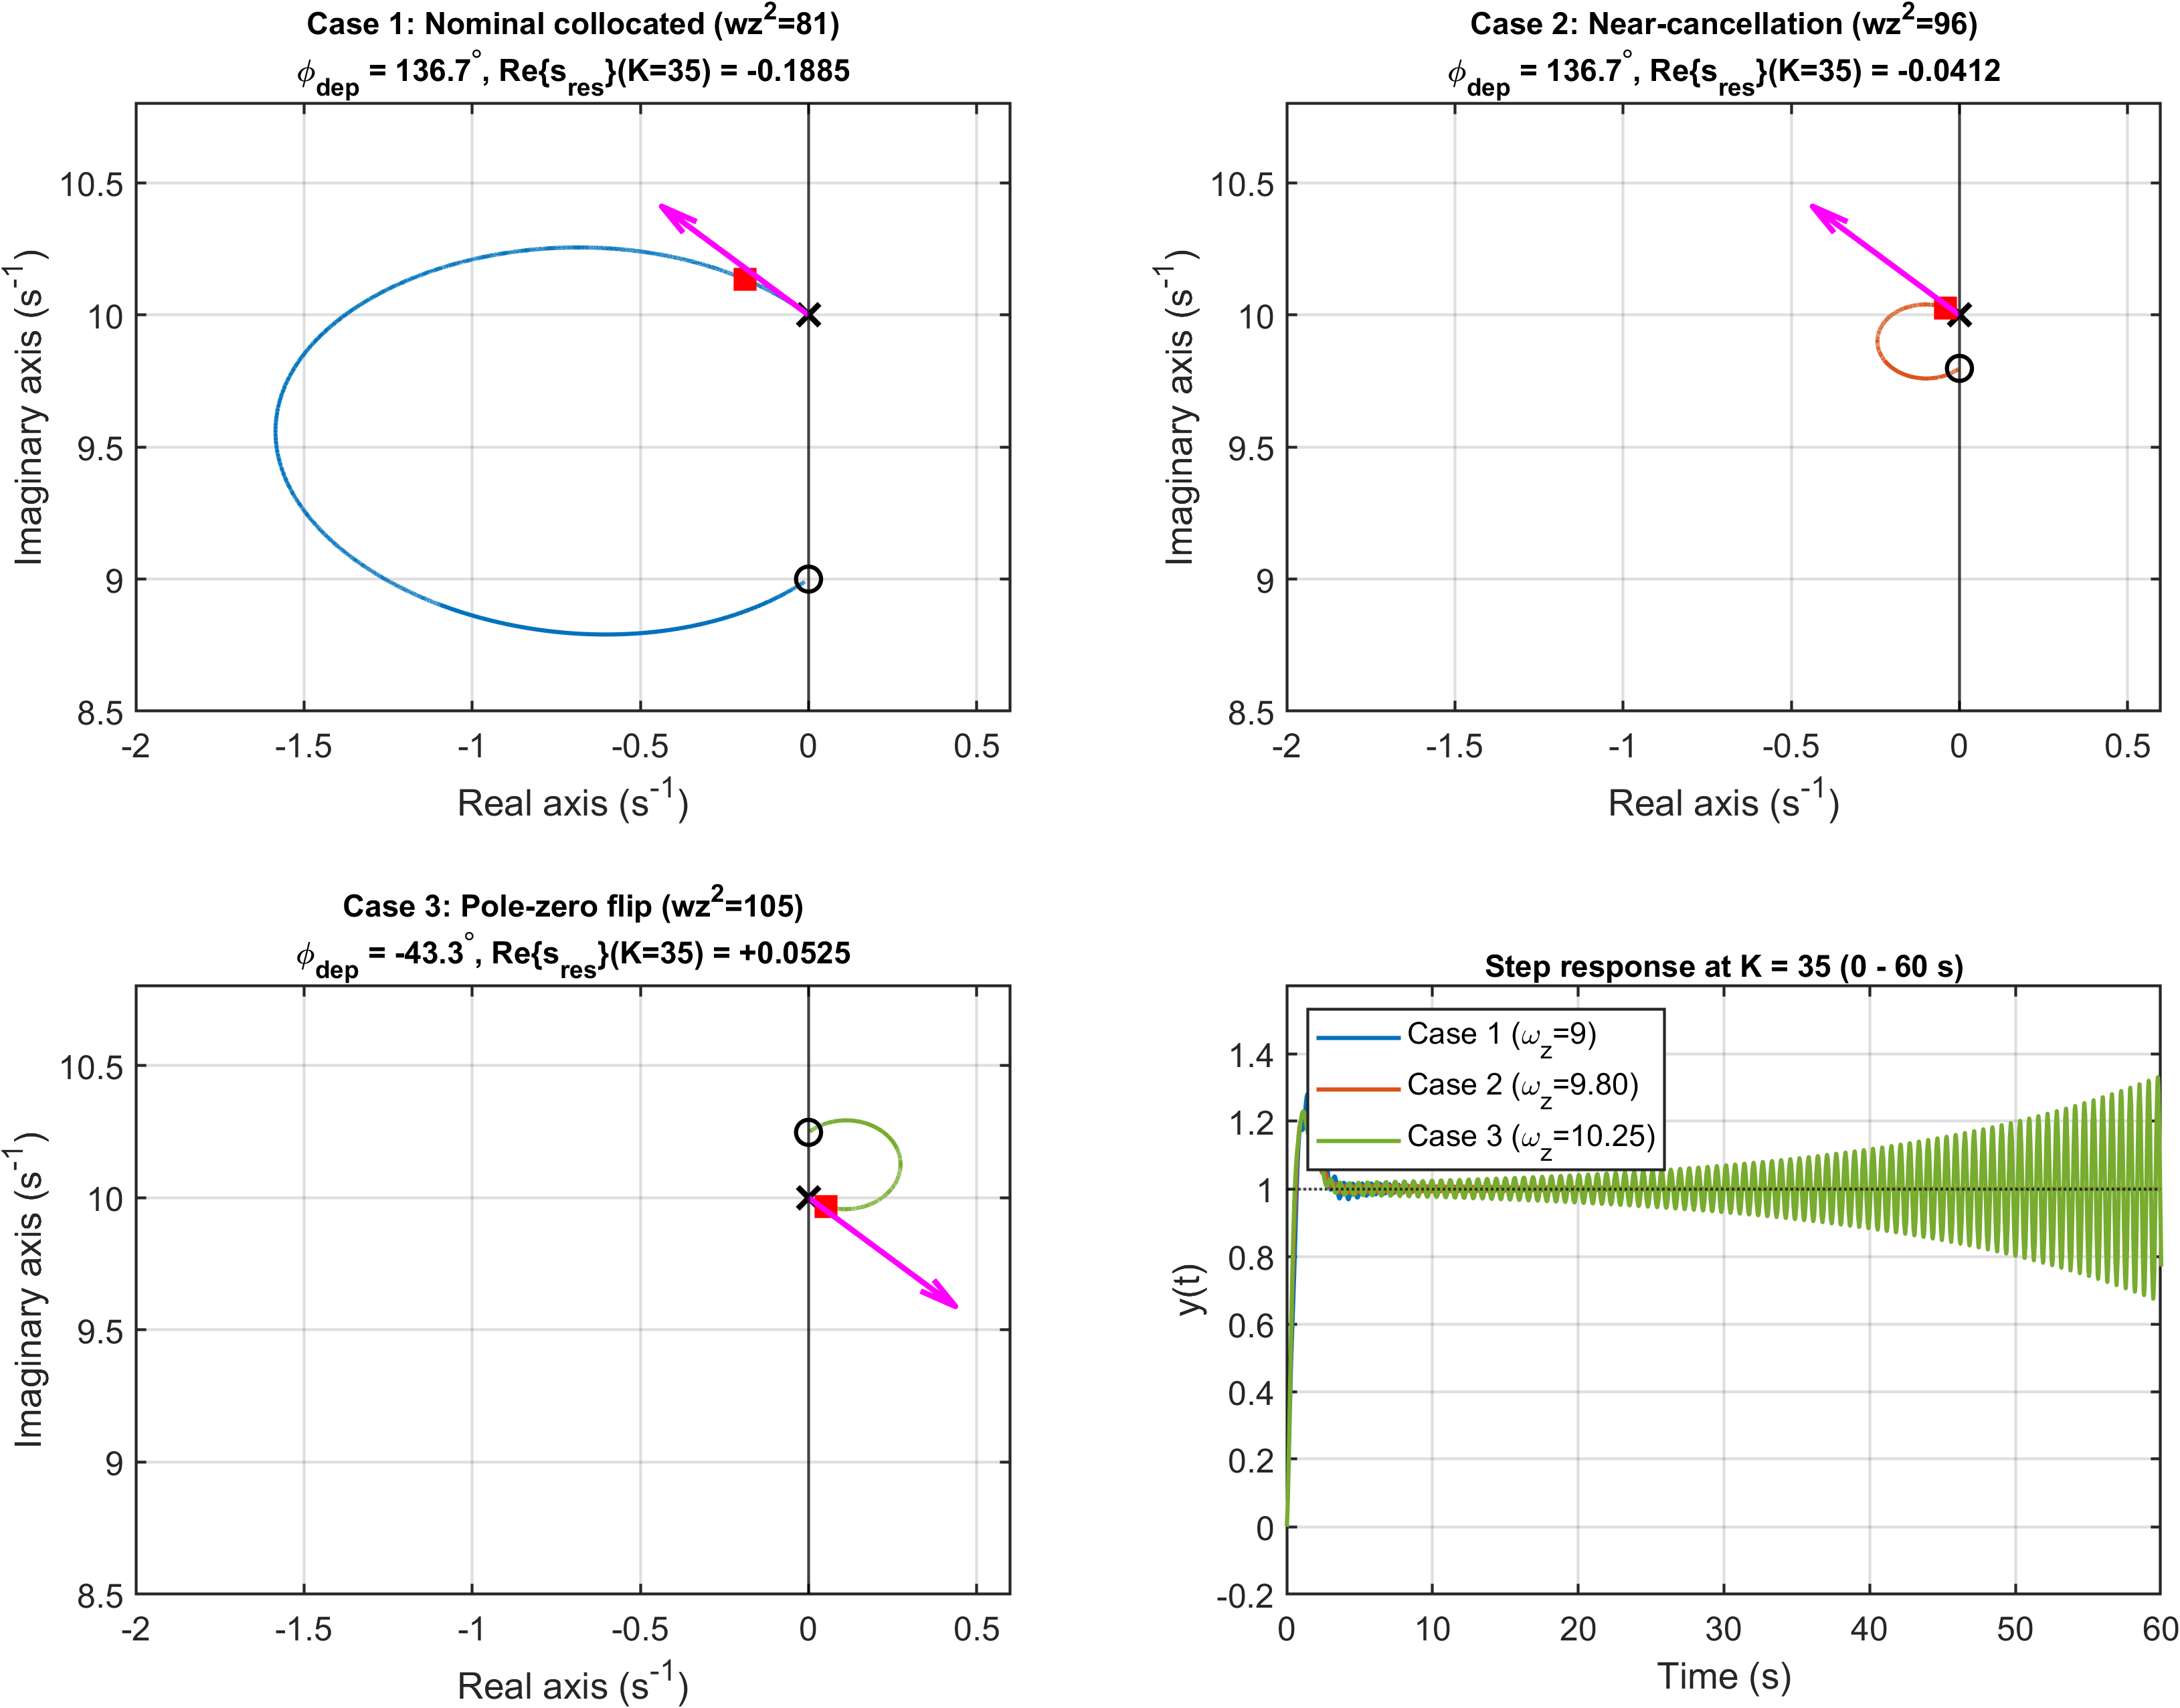
\includegraphics[width=\textwidth]{Fig2_PoleZeroFlip.png}
  \caption{Resonant branch for the three cases (magenta arrow: departure direction; red square: \(K=35\)) and the \(60~\mathrm{s}\) step responses at \(K=35\).}
  \label{fig:flip}
\end{figure}

Case~2 departs at the same angle as Case~1, but its loop is much smaller because the pole and the zero are only \(0.2~\mathrm{rad/s}\) apart.
At \(K=35\) the resonant real part shrinks from \(-0.188\) to \(-0.041\), and \(\zeta_{\mathrm{res}}\) falls from \(0.0186\) to \(0.0041\), a factor of \(4.5\).
Its residue also falls, from \(0.0522\) to \(0.0113\), because the near pole--zero cancellation makes the mode almost invisible from the reference.
The \(2\%\) settling time drops to \(2.878~\mathrm{s}\): the ripple starts inside the band, and the dominant pair, now at \(\zeta=0.826\), sets \(t_s\).
That does not make Case~2 better, however.
The window maxima of \(|y-1|\) are \(9.54\times10^{-3}\) on \([5,10]~\mathrm{s}\), \(4.01\times10^{-3}\) on \([25,30]~\mathrm{s}\), and \(1.18\times10^{-3}\) on \([55,60]~\mathrm{s}\), so a small vibration lingers for more than a minute.
For comparison, Case~1 falls from \(2.07\times10^{-2}\) to \(1.62\times10^{-6}\) over the same windows.

In Case~3 the branch leaves \(+j10\) into the right half-plane and ends at the zero \(+j10.247\), and Figure~\ref{fig:flip} shows the whole loop to the right of the imaginary axis.
No positive gain stabilizes the resonance, and lowering \(K\) only slows the divergence.
At \(K=35\) the dominant pair is well damped (\(\zeta=0.878\)), so the response looks normal for the first few seconds, but the \(9.97~\mathrm{rad/s}\) mode grows as \(e^{+0.0525t}\).
Its window maxima are \(2.42\times10^{-2}\), \(6.87\times10^{-2}\), and \(0.331\).
The ratio between the first two, \(2.835\), agrees with the predicted \(e^{0.05248\times 20}=2.86\).
The same check holds for the decaying cases: Case~1 falls by \(0.0227\) between the first two windows against \(e^{-0.18848\times20}=0.0231\), and Case~2 by \(0.420\) against \(0.439\).

These three cases show that this design depends on the plant's poles and zeros alternating along the imaginary axis.
With \(\omega_z<\omega_p\), the lead compensator damps the mode for every gain, even though only slightly.
If load or sensor placement reverses the pair, the same compensator destabilizes the mode for every gain.
Moving \(\omega_z\) by less than \(5\%\), from \(9.80\) to \(10.25~\mathrm{rad/s}\), is enough to cross that boundary.

%==============================================================================
\section{Extension 2: notch reference pre-filter and control effort}

To remove the ripple without touching the loop, Design~B places a pre-filter \(F(s)\) between \(r\) and the summing junction.
Its zeros sit on the closed-loop resonant pole of Design~A, \(p_r=-0.1885+10.1349j\), and its poles are a well-damped pair at the same frequency:
\begin{equation}
  F(s)=\frac{s^2+2(0.01859)(10.13668)\,s+10.13668^2}{s^2+2(0.70)(10.13668)\,s+10.13668^2},
  \qquad F(0)=F(\infty)=1 .
  \label{eq:F}
\end{equation}
Because \(F\) lies outside the loop, the closed-loop poles, the stability, and the disturbance response are those of Design~A.
Only the map from \(r\) changes, to \(T(s)F(s)\) and \(M(s)F(s)\).
The residue of \(p_r\) in \(TF\) is \(9.8\times10^{-17}\), which is zero to machine precision.

\begin{table}[H]
  \centering
  \caption{Unit-step output and control effort, \(0\le t\le 6~\mathrm{s}\), \(K=35\). The drift row applies the nominal \(F(s)\) to the Case~2 plant (\(\omega_z^2=96\)) without retuning it.}
  \label{tab:pf}
  \small
  \setlength{\tabcolsep}{4pt}
  \begin{tabular}{lcccccc}
    \toprule
    Design & \%OS & \(t_s\) & \(\max|y-1|_{[4,6]}\) & \(u(0^+)\) & \(u_{\mathrm{RMS},[0,6]}\) & \(u_{\mathrm{RMS},[3,6]}\) \\
    \midrule
    A: lead only & \(28.17\%\) & \(5.497~\mathrm{s}\) & \(3.13\times10^{-2}\) & \(35.00\) & \(2.980\) & \(0.3466\) \\
    B: lead \(+\) \(F(s)\) & \(23.83\%\) & \(3.252~\mathrm{s}\) & \(7.60\times10^{-3}\) & \(35.00\) & \(2.232\) & \(0.0650\) \\
    B on drifted plant & \(21.84\%\) & \(3.055~\mathrm{s}\) & \(2.44\times10^{-3}\) & \(35.00\) & \(2.192\) & \(0.0350\) \\
    \bottomrule
  \end{tabular}
\end{table}

\begin{figure}[H]
  \centering
  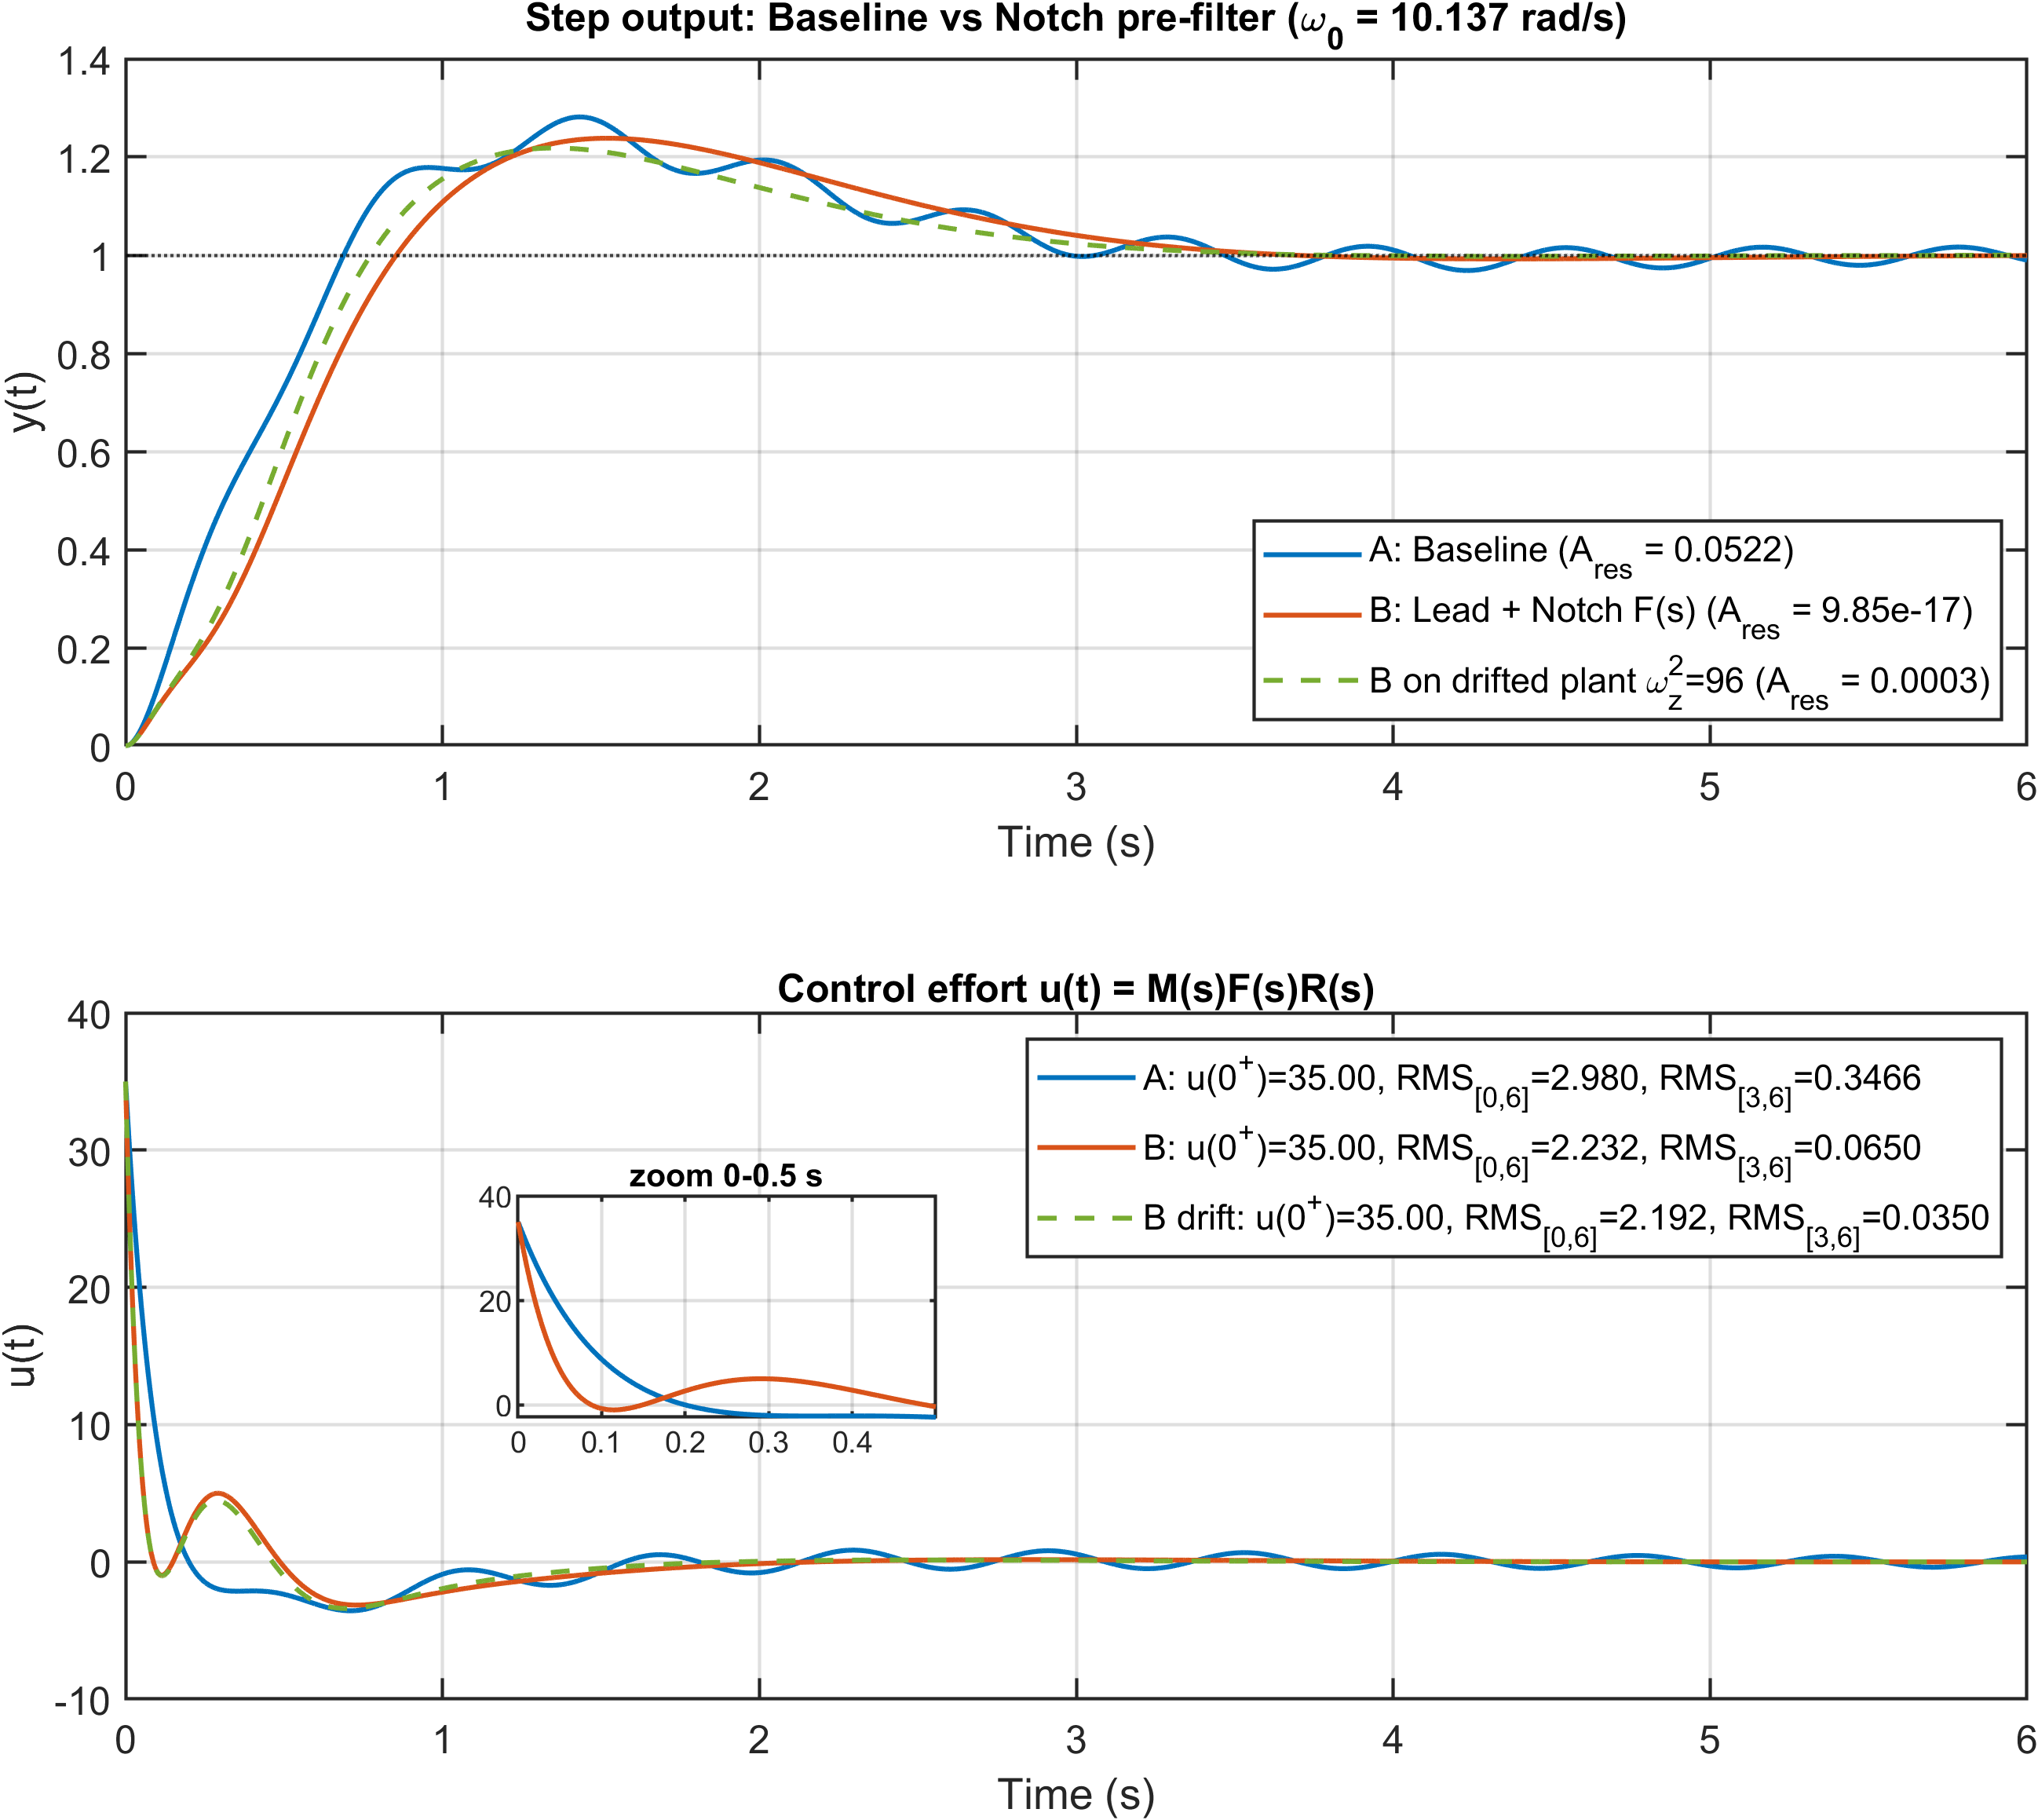
\includegraphics[width=0.92\textwidth]{Fig3_NotchPrefilter.png}
  \caption{Top: step output for Designs A and B and for B on the drifted plant. Bottom: control input, with the first \(0.5~\mathrm{s}\) enlarged.}
  \label{fig:pf}
\end{figure}

The pre-filter removes the ripple from the output.
The \(2\%\) settling time falls from \(5.497\) to \(3.252~\mathrm{s}\), a \(41\%\) reduction, because \(t_s\) was set by the vibration in~\eqref{eq:tsenv}.
The overshoot falls from \(28.2\%\) to \(23.8\%\), which is close to the \(24.5\%\) of the reduced model in Table~\ref{tab:os}, as expected once the resonant contribution has been removed.
The late error \(\max|y-1|\) on \([4,6]~\mathrm{s}\) drops by a factor of \(4.1\). What remains is the tail of the dominant pair, not vibration.
On the actuator, the RMS of \(u\) after \(3~\mathrm{s}\) drops from \(0.347\) to \(0.065\), a factor of \(5.3\), and the RMS over the whole window drops by \(25\%\).

The pre-filter does not reduce the initial kick.
Because \(G\) is strictly proper, with relative degree two, \(M(s)=D/(1+DG)\to K\) as \(s\to\infty\), so
\begin{equation}
  u(0^+)=\lim_{s\to\infty}M(s)F(s)=K\cdot F(\infty)=35
  \label{eq:u0}
\end{equation}
for both designs, as Table~\ref{tab:pf} shows.
The enlarged plot shows how B redistributes this effort: the kick decays faster and is followed by a second positive pulse near \(0.3~\mathrm{s}\), which delays the rise slightly.
To lower \(u(0^+)\), \(F\) would need \(F(\infty)<1\), for example an extra low-pass factor, or the gain would have to come down.

The drift row tests a pre-filter left tuned for the nominal plant.
Without the filter, the drifted plant alone has \(A_{\mathrm{res}}=0.0113\). With the nominal filter that falls to \(2.95\times10^{-4}\), a factor of \(38\), even though the filter is tuned to \(10.137~\mathrm{rad/s}\) and the drifted resonance is at \(10.027~\mathrm{rad/s}\).
This test is easier than it looks, because the drift has already weakened the mode.
It also has a clear limit: no pre-filter can help Case~3, where the instability is in the loop itself.

Design~B also leaves three things unchanged.
The resonant pole keeps \(\zeta=0.0186\), so a torque disturbance at the plant input, sensor noise, or a nonzero initial deflection excites the same lightly damped ringing as before.
The cancellation in \(TF\) depends on knowing \(p_r\), so the filter has to be retuned whenever the plant is.
A filter zero damping of \(0.0186\) also means the notch is very narrow.

%==============================================================================
\section{Conclusion}

For the textbook question, the lead compensator stabilizes the flexible loop for every \(K>0\), and \(K_{\mathrm{opt}}=32.57\) gives the dominant pair exactly \(\zeta=0.707\). The textbook's \(K\approx35\) is a graphical estimate that gives \(\zeta=0.739\).
No gain gives every root \(\zeta>0.5\): the resonant branch is a closed loop between \(+j10\) and \(+j9\), and its damping never exceeds \(0.164\).
The step response at \(K=35\) overshoots by \(28\%\), not the \(3\%\) a second-order model predicts, mainly because of the closed-loop zero at \(-1\). Its \(5.5~\mathrm{s}\) settling time is set by the \(10~\mathrm{rad/s}\) ripple, not by the dominant poles.

For the extension, the result that matters most for implementation is the pole--zero ordering.
Moving the antiresonance from below the resonance to above it subtracts exactly \(180^\circ\) from the departure angle, and the same compensator then destabilizes the mode for every gain.
A shift of less than \(5\%\) in \(\omega_z\) is enough to cause this.
Any physical change that can reverse the order, such as moving the sensor away from the actuator, has to be ruled out before this compensator is used.
The notch pre-filter is a cheap fix for the reference response only. It cuts the settling time by \(41\%\) and the late actuator chatter by a factor of \(5\), but leaves \(u(0^+)=35\), the loop damping, and the disturbance response unchanged.
Damping the mode itself would require a change inside the loop, for example a phase-stabilizing notch or added structural damping.
\end{document}
